% =============================================================================
% Kapitel 3: Methodik
% =============================================================================
\chapter{Methodik}
\label{ch:methodik}

\textcolor{red}{
    \begin{itemize}
        \item verschiedene modelle gegenüberstellen
        \item finetuning von modellen
        \item datenlage
        \item preprocessing von daten
        \item behandlung von sonderbaren werten (entfernen, stärker repräsentieren, etc.)
        \item robustheit von modell testen/erhöhen
        \item ausgesuchtes netz anpassen, architektur anpassen, etc.
        \item erklärung für modelle, versuche usw
    \end{itemize}
}

Das Ziel der Methodik ist es, die zuvor genannten Forschungsfragen in \cref{sec:forschungsfragen} zu beantworten. Um dies zu erreichen, werden im Folgenden die methodischen Schritte beschrieben, die dafür durchgeführt werden. Die Methodik umfasst die Auswahl und Implementierung von Datenaufbereitung und Machine-Learning-Modellen, die Gegenüberstellung der Modelle, sowie die Durchführung von Ablationsexperimenten, um die besten Modelle zu identifizieren. Die Methodik ist in \cref{fig:methodik} schematisch dargestellt. Der Arbeitsfluss beginnt mit der Auswahl und Aufbereitung der Daten -- in diesem Fall fünf verschiedene Datenquellen -- welche in ein einheitliches Schema transformiert werden. Anschließen werden die Daten auf ihre Qualität hin bewertet und relevante Features extrahiert. Anschließend werden die Daten in zwei Modellfamilien eingespeist: Klassifikator und Zeitreihenprognose. Die Modelle werden dann in einem experimentellen Design evaluiert, das sowohl die Isolation von Daten- und Algorithmen-Effekten als auch eine Ablationsstudie umfasst. Abschließend werden die Ergebnisse bewertet und die Forschungsfragen beantwortet. 

\begin{figure}[htbp]
  \centering
  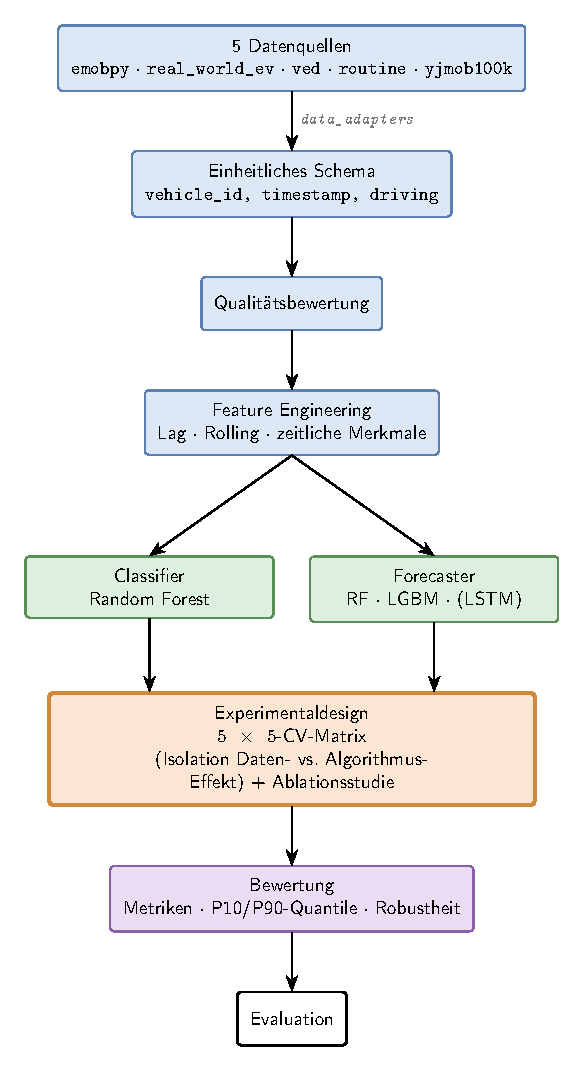
\includegraphics[width=0.7\textwidth]{graphen/methodik/methodik_workflow.pdf}
  \caption{Schematischer Workflow der Methodik: von den fünf Datenquellen über
    den geteilten Feature-Kern und die beiden Modellfamilien bis zum
    Experimentaldesign und der Bewertung.}
  \label{fig:methodik}
\end{figure}

Die Arbeit lässt sich in drei große Teile gliedern:
\begin{itemize}
    \item \textbf{Datenaufbereitung}: Das Erkundschaften der Datenlandschaft, die Transformation der Daten in ein geeignetes Format und die Auswahl relevanter Features.
    \item \textbf{Machine Learning}: Die Auswahl und Implementierung verschiedener Machine-Learning-Modelle auf Grund ihrer unterschiedlichen Eigenschaften (leaf- und level-wise Wachstum, Bagging und Boosting, modellierte zeitliche Abhängigkeiten).
    \item \textbf{Ablationsexperimente}: Im Rahmen einer Ablationstudie werden verschiedene Modelle hinsichtlich ihrer Wertigkeit (in diesem Fall: Vorhersagegenauigkeit, Robustheit, Zuverlässigkeit) miteinander verglichen, um die besten Modelle zu identifizieren. 
\end{itemize}

Es bleibt zu beachten, dass die Ablation nicht unbedingt zur Abtragung aller nicht-primären Modelle führt, sondern eine eventuelle Kooperation von Modellen auch eine Möglichkeit darstellt. 


% -----------------------------------------------------------------------------
\section{Forschungsdesign}
\label{sec:forschungsdesign}

\todo{Das übergeordnete Forschungsdesign beschreiben (z.\,B.\ qualitativ, quantitativ, Mixed-Methods, Design Science Research, etc.).}

% -----------------------------------------------------------------------------

\section{Untersuchungsablauf}
\label{sec:untersuchungsablauf}

% -----------------------------------------------------------------------------

\section{Datengrundlage und Quellen}
\label{sec:datengrundlage}

% -----------------------------------------------------------------------------

\section{Feature Engineering}
\label{sec:feature}

% -----------------------------------------------------------------------------

\section{Modellauswahl}
\label{sec:modellauswahl}

% -----------------------------------------------------------------------------

\section{Experimentaldesign}
\label{sec:experimentaldesign}

% -----------------------------------------------------------------------------

\section{Bewertung}
\label{sec:bewertung}


